%----------------------------------------------------------------------------
\chapter{Felhasználói dokumentáció}
%----------------------------------------------------------------------------

\section{Kezdőoldal}
Az oldal látogatóit egy üdvözlőszöveg köszönti, amely röviden összefoglalja a felhasználó lehetőségeit az oldalon.
Amennyiben nem szeretne a felhasználó egy új profilt létrehozni, vagy bejelentkezni, akkor lehetősége van elnavigálni a tanulói felületre, ahol szabadon böngészheti a jelen levő kriptográfiai rendszereket.
Viszont, ha a felhasználó él a bejelentkezés lehetőségével, akkor hozzáférése lesz a műveletek elvégzéséért felelős felülethez is.
Továbbá minden oldalon jelen van, egy nyelv választó, mely lehetőséget ad, hogy a felhasználó más nyelven is böngészhessen a platformon (\ref{fig:langSelector}).


\section{Tanulói felület}
A tanulói felület bal oldalán egy menün keresztül lehet navigálni a módszerek között, a kiválasztás után megjelenik 2 gomb (vissza, következő), amely segít az adott rendszerhez tartozó tartalom navigálásásában.
Ha a felhasználó úgy dönt, hogy mégis hozzáférést szeretne az oldal többi funkciójához, akkor ezt a belépés fülre kattintva, egy gyors bejelentkezés vagy új profil létrehozása után megkapja.



\section{Crypt felület}
A Crypt felületen lehet kipróbálni a rendszerbe beépített kriptográfiai műveleteket, ehhez rendelkezésre áll egy kiválasztó, ahol jelen vannak az elérhető lehetőségek. A választás után megjelenhet bizonyos számú beviteli mező, ezek a kiválasztott művelet bemeneti paramétereit várják (\ref{fig:aesDeOpt}).
Egy művelet sikeres elvégzése után az előzmények táblában megjelenik az eredmény, ezt megelőzően pedig a felhasználó által végrehajtott műveletek előzményei (\ref{fig:cryptBase}).


\newpage
\begin{figure}[!h]
	\centering
	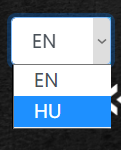
\includegraphics[scale=1]{images/langSelector}
	\caption{Nyelvválasztó}
	\label{fig:langSelector}
\end{figure}

\begin{figure}[!h]
	\centering
	
\includegraphics[scale=0.5]{images/aesDeOptions}
	\caption{Példa beviteli mezőre - AES-128 CTR DE}
	\label{fig:aesDeOpt}
\end{figure}

\begin{figure}[!h]
	\centering
	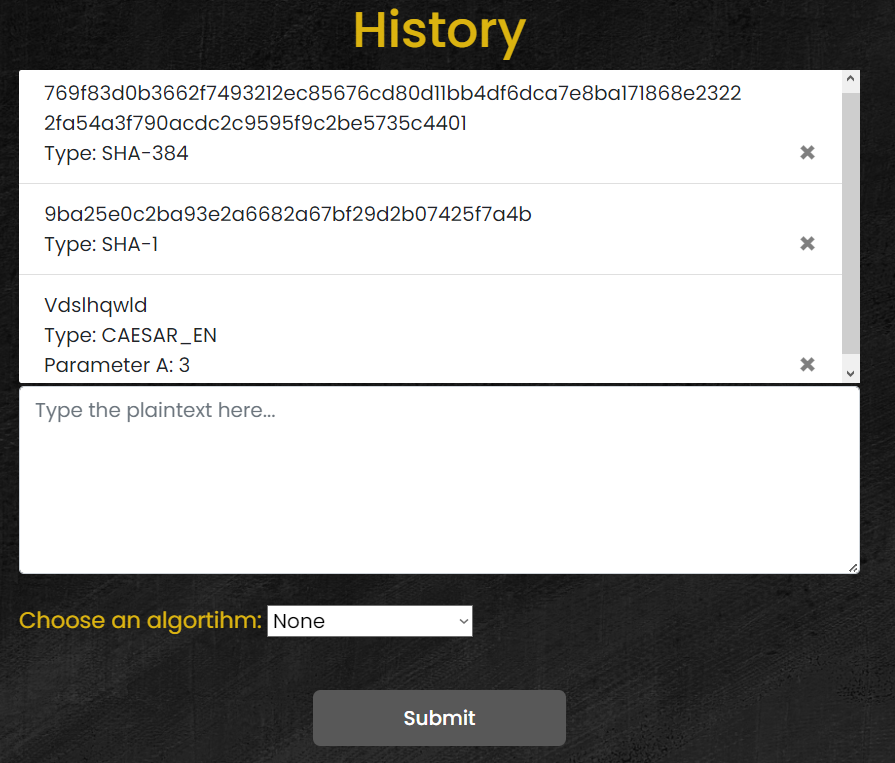
\includegraphics[scale=0.45]{images/cryptBase}
	\caption{Crypt felület}
	\label{fig:cryptBase}
\end{figure}
